% questions.tex —— 2003 年·春季北京卷·文科 · 题目内容片段（无答案）
% 由 tools/generate_projects.py 依来源总账自 2003/2003_数学真题_春季北京文_试题.md 生成，勿手改（改源 MD 后重跑）


\begin{gktip}
\textbf{来源说明}：题签、题面和印刷页码依据固定 PDF \texttt{春季高考/2003/2003春季北京文.pdf} 核对。文件 SHA-256 与来源清单一致，PDF 共 2 页，印刷页码为 121–122；对应的上游 Git blob 在书源仓库中存在。该 PDF 是 XeTeX 排印副本，并非原卷扫描。现已按题签登记为本库内部 canonical 输入；此绑定只表示本库选用该固定副本，不认证其发布者、版次、来源链或官方身份。

\textbf{转录说明}：使用 PDF 原生文字层辅助定位，不调用 OCR；PDF 第 1、2 页已逐页目视核对。题面共有 22 题：第 1–12 题单项选择，第 13–16 题填空，第 17–22 题解答。表格空格保留为空白；所有图均以 TikZ 源码重绘，未提交原卷截图。

\textbf{答案说明}：固定源文件只含试题页，没有答案页；本稿仅转录题面，\texttt{official_answer} 保持 \texttt{null}。本库另有独立推导的答案与解析稿，明确标记为非官方。

\textbf{图表说明}：第 9、11、14、19、22 题的矢量图稿均为按原图结构重绘的示意图，不把扫描图比例当作精确数学条件；Q15 数据以排版表格保留，不以图片代替。逐项边界见图表清单。
\end{gktip}

\gkpart{一、选择题}

\begin{question}
\gkti{1}设 $a,b,c,d\in\mathbb{R}$，且 $a>b$、$c>d$，则下列结论中正确的是\mbox{（　　）}。

（A）$a+c>b+d$　　（B）$a-c>b-d$　　（C）$ac>bd$　　（D）$\dfrac{a}{d}>\dfrac{b}{c}$。

\end{question}
\begin{question}
\gkti{2}设 $M$ 和 $m$ 分别表示函数 $y=\dfrac13\cos x-1$ 的最大值和最小值，则 $M+m$ 等于\mbox{（　　）}。

（A）$\dfrac23$　　（B）$-\dfrac23$　　（C）$-\dfrac43$　　（D）$-2$。

\end{question}
\begin{question}
\gkti{3}若 $f(x)=\dfrac{x-1}{x}$，则方程 $f(4x)=x$ 的根是\mbox{（　　）}。

（A）$-2$　　（B）$2$　　（C）$-\dfrac12$　　（D）$\dfrac12$。

\end{question}
\begin{question}
\gkti{4}若集合 $M=\{y\mid y=2^{-x}\}$，$P=\{y\mid y=\sqrt{x-1}\}$，则 $M\cap P=$\mbox{（　　）}。

（A）$\{y\mid y>1\}$　　（B）$\{y\mid y\ge1\}$　　（C）$\{y\mid y>0\}$　　（D）$\{y\mid y\ge0\}$。

\end{question}
\begin{question}
\gkti{5}若 $A,B,C$ 是 $\triangle ABC$ 的三个内角，且 $A<B<C$（$C\ne\dfrac\pi2$），则下列结论中正确的是\mbox{（　　）}。

（A）$\tan A<\tan C$　　（B）$\cot A<\cot C$　　（C）$\sin A<\sin C$　　（D）$\cos A<\cos C$。

\end{question}
\begin{question}
\gkti{6}在等差数列 $\{a_n\}$ 中，已知 $a_1+a_2+a_3+a_4+a_5=20$，那么 $a_3$ 等于\mbox{（　　）}。

（A）$4$　　（B）$5$　　（C）$6$　　（D）$7$。

\end{question}
\begin{question}
\gkti{7}设复数 $z_1=-1+i$，$z_2=\dfrac12+\dfrac{\sqrt3}{2}i$，则 $\arg\dfrac{z_1}{z_2}=$\mbox{（　　）}。

（A）$-\dfrac5{12}\pi$　　（B）$\dfrac5{12}\pi$　　（C）$\dfrac7{12}\pi$　　（D）$\dfrac{13}{12}\pi$。

\end{question}
\begin{question}
\gkti{8}函数 $f(x)=|x|$ 和 $g(x)=x(2-x)$ 的递增区间依次是\mbox{（　　）}。

（A）$(-\infty,0]$、$(-\infty,1]$　　（B）$(-\infty,0]$、$[1,+\infty)$

（C）$[0,+\infty)$、$(-\infty,1]$　　（D）$[0,+\infty)$、$[1,+\infty)$。

\Needspace{0.4\textheight}
\end{question}
\begin{question}
\gkti{9}在同一坐标系中，方程 $a^2x^2+b^2y^2=1$ 与 $ax+by^2=0$（$a>b>0$）的曲线大致是\mbox{（　　）}。
\nopagebreak[4]
\begin{center}% Q9: preserve the four qualitative alternatives from the fixed scan.
% Curve scales are schematic; only axes, orientations, and opening directions matter.
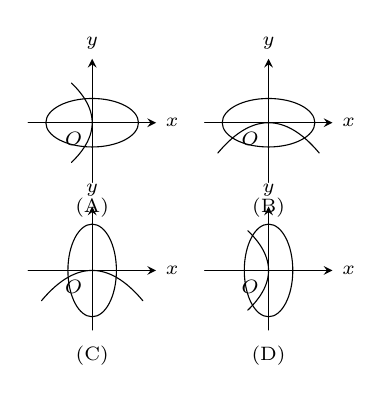
\begin{tikzpicture}[
  x=0.56cm,y=0.56cm,line cap=round,line join=round,>=stealth,
  every node/.style={font=\scriptsize}
]
\def\axes{%
  \draw[->] (-1.45,0)--(1.45,0) node[right] {$x$};
  \draw[->] (0,-1.35)--(0,1.45) node[above] {$y$};
  \node[below left] at (0,0) {$O$};
}
\def\leftparabola{%
  \draw[domain=-0.9:0.9,samples=60,variable=\t]
    plot ({-0.58*\t*\t},{\t});
}
\def\downparabola{%
  \draw[domain=-1.15:1.15,samples=60,variable=\t]
    plot ({\t},{-0.52*\t*\t});
}
\begin{scope}[shift={(0,0)}]
  \axes
  \draw (0,0) ellipse [x radius=1.05,y radius=0.55];
  \leftparabola
  \node[below] at (0,-1.48) {(A)};
\end{scope}
\begin{scope}[shift={(4,0)}]
  \axes
  \draw (0,0) ellipse [x radius=1.05,y radius=0.55];
  \downparabola
  \node[below] at (0,-1.48) {(B)};
\end{scope}
\begin{scope}[shift={(0,-3.35)}]
  \axes
  \draw (0,0) ellipse [x radius=0.55,y radius=1.05];
  \downparabola
  \node[below] at (0,-1.48) {(C)};
\end{scope}
\begin{scope}[shift={(4,-3.35)}]
  \axes
  \draw (0,0) ellipse [x radius=0.55,y radius=1.05];
  \leftparabola
  \node[below] at (0,-1.48) {(D)};
\end{scope}
\end{tikzpicture}
\end{center}
\nopagebreak[4]
\end{question}
\begin{question}
\gkti{10}某班新年联欢会原定的 $5$ 个节目已排成节目单，开演前又增加了两个新节目。如果将这两个节目插入原节目单中，且两个新节目不相邻，那么不同插法的种数为\mbox{（　　）}。

（A）$6$　　（B）$12$　　（C）$15$　　（D）$30$。

\Needspace{0.4\textheight}
\end{question}
\begin{question}
\gkti{11}如图，在正三角形 $ABC$ 中，$D,E,F$ 分别为各边的中点，$G,H,I,J$ 分别为 $AF,AD,BE,DE$ 的中点。将 $\triangle ABC$ 沿 $DE,EF,DF$ 折成三棱锥以后，$GH$ 与 $IJ$ 所成角的度数为\mbox{（　　）}。
\nopagebreak[4]
\begin{center}% Q11: flat subdivision of the equilateral triangle before folding.
% Coordinates enforce the stated midpoints; they do not encode a perspective after folding.
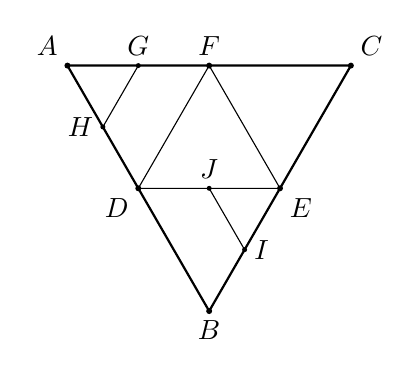
\begin{tikzpicture}[scale=0.9,line cap=round,line join=round]
  \coordinate (A) at (0,3.4641);
  \coordinate (C) at (4,3.4641);
  \coordinate (B) at (2,0);
  \coordinate (D) at (1,1.73205);
  \coordinate (E) at (3,1.73205);
  \coordinate (F) at (2,3.4641);
  \coordinate (G) at (1,3.4641);
  \coordinate (H) at (0.5,2.59808);
  \coordinate (I) at (2.5,0.86603);
  \coordinate (J) at (2,1.73205);

  \draw[thick] (A)--(C)--(B)--cycle;
  \draw (D)--(E)--(F)--cycle;
  \draw (G)--(H) (J)--(I);

  \fill (A) circle (1.2pt) node[above left] {$A$};
  \fill (B) circle (1.2pt) node[below] {$B$};
  \fill (C) circle (1.2pt) node[above right] {$C$};
  \fill (D) circle (1.2pt) node[below left] {$D$};
  \fill (E) circle (1.2pt) node[below right] {$E$};
  \fill (F) circle (1.2pt) node[above] {$F$};
  \fill (G) circle (1pt) node[above] {$G$};
  \fill (H) circle (1pt) node[left] {$H$};
  \fill (I) circle (1pt) node[right] {$I$};
  \fill (J) circle (1pt) node[above] {$J$};
\end{tikzpicture}
\end{center}
\nopagebreak[4]
（A）$90^\circ$　　（B）$60^\circ$　　（C）$45^\circ$　　（D）$0^\circ$。

\end{question}
\begin{question}
\gkti{12}已知直线 $ax+by+c=0$（$abc\ne0$）与圆 $x^2+y^2=1$ 相切，则三条边长分别为 $|a|,|b|,|c|$ 的三角形\mbox{（　　）}。

（A）是锐角三角形　　（B）是直角三角形　　（C）是钝角三角形　　（D）不存在。

\end{question}
\gkpart{二、填空题}

\begin{question}
\gkti{13}函数 $y=\sin 2x+1$ 的最小正周期为\underline{\qquad}。

\Needspace{0.4\textheight}
\end{question}
\begin{question}
\gkti{14}如图，一个底面半径为 $R$ 的圆柱形量杯中装有适量的水。若放入一个半径为 $r$ 的实心铁球，水面高度恰好升高 $r$，则 $\dfrac Rr=$\underline{\qquad}。
\nopagebreak[4]
\begin{center}% Q14: schematic side-by-side level comparison; not to scale.
\begin{tikzpicture}[scale=0.9,line cap=round,line join=round,>=stealth]
  % Initial cylindrical cup and water level.
  \fill[black!12] (0,0)--(1.5,0)--(1.5,1.15)--(0,1.15)--cycle;
  \draw (0,0)--(0,3.0) (1.5,0)--(1.5,3.0) (0,0)--(1.5,0);
  \draw (-0.08,3.0)--(0.12,3.0) (1.38,3.0)--(1.58,3.0);
  \draw (0,1.15)--(1.5,1.15);

  % Same cup after the sphere is submerged; the free surface rises by r.
  \fill[black!12] (3,0)--(4.5,0)--(4.5,1.85)--(3,1.85)--cycle;
  \draw[fill=white] (3.75,0.68) circle (0.68);
  \draw (3,0)--(3,3.0) (4.5,0)--(4.5,3.0) (3,0)--(4.5,0);
  \draw (2.92,3.0)--(3.12,3.0) (4.38,3.0)--(4.58,3.0);
  \draw (3,1.85)--(4.5,1.85);
  \draw (3.75,0.68)--(4.43,0.68) node[midway,above] {$r$};

  % Increase in level is exactly the sphere radius r.
  \draw[<->] (2.55,1.15)--(2.55,1.85);
  \node[left] at (2.55,1.5) {$r$};
  \node[below] at (0.75,-0.18) {放入前};
  \node[below] at (3.75,-0.18) {放入后};
\end{tikzpicture}
\end{center}
\nopagebreak[4]
\end{question}
\begin{question}
\gkti{15}在某报《自测健康状况》的报道中，自测血压结果与相应年龄的统计数据如下表。观察表中数据的特点，用适当的数填入表中空白内。

\begin{center}
\begingroup\setlength{\tabcolsep}{4pt}
\begin{tabular}{lrrrrrrrr}
\toprule
年龄（岁） & 30 & 35 & 40 & 45 & 50 & 55 & 60 & 65 \\
\midrule
收缩压（水银柱/毫米） & 110 & 115 & 120 & 125 & 130 & 135 & $\underline{\qquad}$ & 145 \\
舒张压（水银柱/毫米） & 70 & 73 & 75 & 78 & 80 & 83 & $\underline{\qquad}$ & 88 \\
\bottomrule
\end{tabular}
\endgroup
\end{center}

\end{question}
\begin{question}
\gkti{16}已知 $F_1,F_2$ 分别为椭圆 $\dfrac{x^2}{a^2}+\dfrac{y^2}{b^2}=1$ 的左、右焦点，点 $P$ 在椭圆上，$\triangle POF_2$ 是面积为 $\sqrt3$ 的正三角形，则 $b^2$ 的值是\underline{\qquad}。

\end{question}
\gkpart{三、解答题}

\begin{question}
\gkti{17}解不等式：$\log_2(x^2-x-2)>\log_2(2x-2)$。

\end{question}
\begin{question}
\gkti{18}已知函数
\nopagebreak[4]
\[
f(x)=\frac{6\cos^4x-5\cos^2x+1}{\cos 2x},
\]
求 $f(x)$ 的定义域，判断它的奇偶性，并求其值域。

\Needspace{0.4\textheight}
\end{question}
\begin{question}
\gkti{19}如图，$ABCD-A_1B_1C_1D_1$ 是正四棱柱，侧棱长为 $1$，底面边长为 $2$，$E$ 是棱 $BC$ 的中点。

（1）求三棱锥 $D_1-DBC$ 的体积；

（2）证明 $BD_1\parallel\text{\text{平面} }C_1DE$；

（3）求面 $C_1DE$ 与面 $CDE$ 所成二面角的正切值。
\nopagebreak[4]
\begin{center}% Q19: orthographic schematic with hidden edges dashed; projection is not to scale.
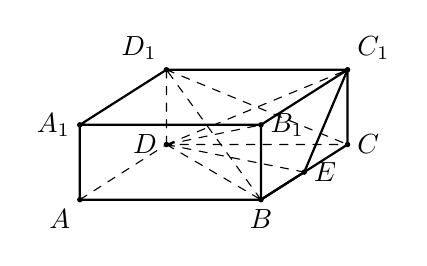
\begin{tikzpicture}[
  x={(1.15cm,0cm)},y={(0.55cm,0.35cm)},z={(0cm,0.95cm)},
  line cap=round,line join=round,>=stealth
]
  \coordinate (A) at (0,0,0);
  \coordinate (B) at (2,0,0);
  \coordinate (C) at (2,2,0);
  \coordinate (D) at (0,2,0);
  \coordinate (A1) at (0,0,1);
  \coordinate (B1) at (2,0,1);
  \coordinate (C1) at (2,2,1);
  \coordinate (D1) at (0,2,1);
  \coordinate (E) at (2,1,0);

  % Rear base edges and the rear vertical are hidden.
  \draw[dashed] (A)--(D)--(C) (D)--(D1);
  % Outer prism edges.
  \draw[thick] (A)--(B)--(C) (A)--(A1)--(B1)--(B)
    (A1)--(D1)--(C1)--(B1) (C)--(C1);
  % Spatial construction lines shown in the source sketch.
  \draw[dashed] (B)--(D1) (D)--(B1) (D)--(E) (D)--(C1) (D)--(B) (D1)--(C);
  \draw[thick] (C1)--(E) (B)--(E);

  \fill (A) circle (1pt) node[below left] {$A$};
  \fill (B) circle (1pt) node[below] {$B$};
  \fill (C) circle (1pt) node[right] {$C$};
  \fill (D) circle (1pt) node[left] {$D$};
  \fill (A1) circle (1pt) node[left] {$A_1$};
  \fill (B1) circle (1pt) node[right] {$B_1$};
  \fill (C1) circle (1pt) node[above right] {$C_1$};
  \fill (D1) circle (1pt) node[above left] {$D_1$};
  \fill (E) circle (1pt) node[right] {$E$};
\end{tikzpicture}
\end{center}
\nopagebreak[4]
\end{question}
\begin{question}
\gkti{20}设 $A(-c,0)$、$B(c,0)$（$c>0$）为两定点，动点 $P$ 到 $A$ 点的距离与到 $B$ 点的距离的比为定值 $a$（$a>0$），求 $P$ 点的轨迹。

\end{question}
\begin{question}
\gkti{21}某租赁公司拥有汽车 $100$ 辆。当每辆车的月租金为 $3000$ 元时，可全部租出。当每辆车的月租金每增加 $50$ 元时，未租出的车将会增加一辆。租出的车每辆每月需要维护费 $150$ 元，未租出的车每辆每月需要维护费 $50$ 元。

（1）当每辆车的月租金定为 $3600$ 元时，能租出多少辆车？

（2）当每辆车的月租金定为多少元时，租赁公司的月收益最大？最大月收益是多少？

\Needspace{0.4\textheight}
\end{question}
\begin{question}
\gkti{22}如图，在边长为 $l$ 的等边 $\triangle ABC$ 中，圆 $O_1$ 为 $\triangle ABC$ 的内切圆，圆 $O_2$ 与圆 $O_1$ 外切，且与 $AB,BC$ 相切，……圆 $O_{n+1}$ 与圆 $O_n$ 外切，且与 $AB,BC$ 相切，如此无限继续下去。记圆 $O_n$ 的面积为 $a_n$（$n\in\mathbb{N}$）。

（1）证明 $\{a_n\}$ 是等比数列；

（2）求 $\displaystyle\lim_{n\to\infty}(a_1+a_2+\cdots+a_n)$ 的值。
\nopagebreak[4]
\begin{center}% Q22: the source shows the incircle, its first tangent circle, and the next small circle near B.
% A normalized side length of 6 is used only to lay out the schematic.
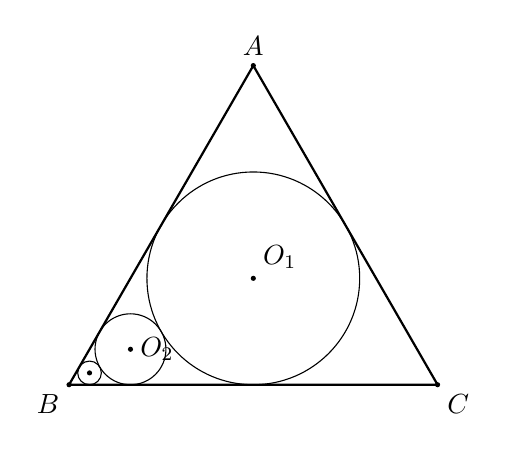
\begin{tikzpicture}[scale=0.78,line cap=round,line join=round]
  \coordinate (A) at (3,5.19615);
  \coordinate (B) at (0,0);
  \coordinate (C) at (6,0);
  \coordinate (Oone) at (3,1.73205);
  \coordinate (Otwo) at (1,0.57735);
  \coordinate (Othree) at (0.33333,0.19245);
  \draw[thick] (A)--(B)--(C)--cycle;
  \draw (Oone) circle (1.73205);
  \draw (Otwo) circle (0.57735);
  \draw (Othree) circle (0.19245);
  \fill (A) circle (1.2pt) node[above] {$A$};
  \fill (B) circle (1.2pt) node[below left] {$B$};
  \fill (C) circle (1.2pt) node[below right] {$C$};
  \fill (Oone) circle (1.2pt) node[above right] {$O_1$};
  \fill (Otwo) circle (1.2pt) node[right] {$O_2$};
  \fill (Othree) circle (1.2pt);
\end{tikzpicture}
\end{center}
\nopagebreak[4]

\end{question}